\documentclass[11pt, a4paper]{article}

\usepackage{geometry} 
\usepackage{epsfig}
\usepackage{epstopdf}
\DeclareGraphicsRule{.tif}{png}{.png}{`convert #1 `dirname #1`/`basename #1 .tif`.png}
\setlength{\oddsidemargin}{0cm}
\setlength{\evensidemargin}{0cm}
\setlength{\topmargin}{-1cm}
\setlength{\textheight}{23cm}
\setlength{\textwidth}{16cm}

\pagestyle{headings}

\newcommand{\BAT}{{\sc BAT}}

%--------------------------------------------------------

\begin{document}

% --------------------------------------------------------
% title
% --------------------------------------------------------

\thispagestyle{empty} 

\begin{figure}
\leftline{
\includegraphics[scale=0.25]{bat.eps} 
\hspace{9.0cm} 
version 0.1} 
\end{figure} 

\title{\BAT\ - A {\sc Bayesian Analysis Toolkit}} 

\author{A.~Caldwell$^{1}$, D.~Kollar${^1}$, K.~Kr\"oninger$^{2}$} 

\maketitle

\begin{center}
$^{1}$~Max-Planck-Institut f\"ur Physik, Munich, Germany \\ 
$^{2}$~II.~Physikalisches Institut, Universit\"at G\"ottingen \\ 
\end{center}

\thispagestyle{empty} 

\begin{abstract} 
The Bayesian Analysis Toolkit, \BAT, is a software package designed to
help solve statistical problems encountered in Bayesian
statistics. Allowing to formulate models and their parameters, the
main purpose of the toolkit is to provide methods to solve the
numerical optimization and integration. It features the possiblity to
estimate parameters and to compare models. A procedure to estimate the
goodness-of-fit is included and based on ensemble tests. 
\end{abstract} 

\pagebreak 

% --------------------------------------------------------
% table of contents 
% --------------------------------------------------------

\thispagestyle{empty} 

\tableofcontents

\pagebreak 

% --------------------------------------------------------
% introduction
% --------------------------------------------------------

\section{Introduction}

The goal of data analysis is to compare model predictions with data,
and draw conclusions on the validity of the model as a representation
of the data, or to estimate best-fit parameter values within the
context of a model. The paradigm for our data analysis package is
shown in Fig.~\ref{fig:scheme}.  Here, the model M can range from a
model purporting to represent nature (e.g., the Standard Model in
particle physics) to a simple parametrization of data useful for
making predictions or for summarizing data.  In the latter case, the
intermediate steps in the figure would be skipped. \\ 

\begin{figure}[htbp] %  figure placement: here, top, bottom, or page
\centering
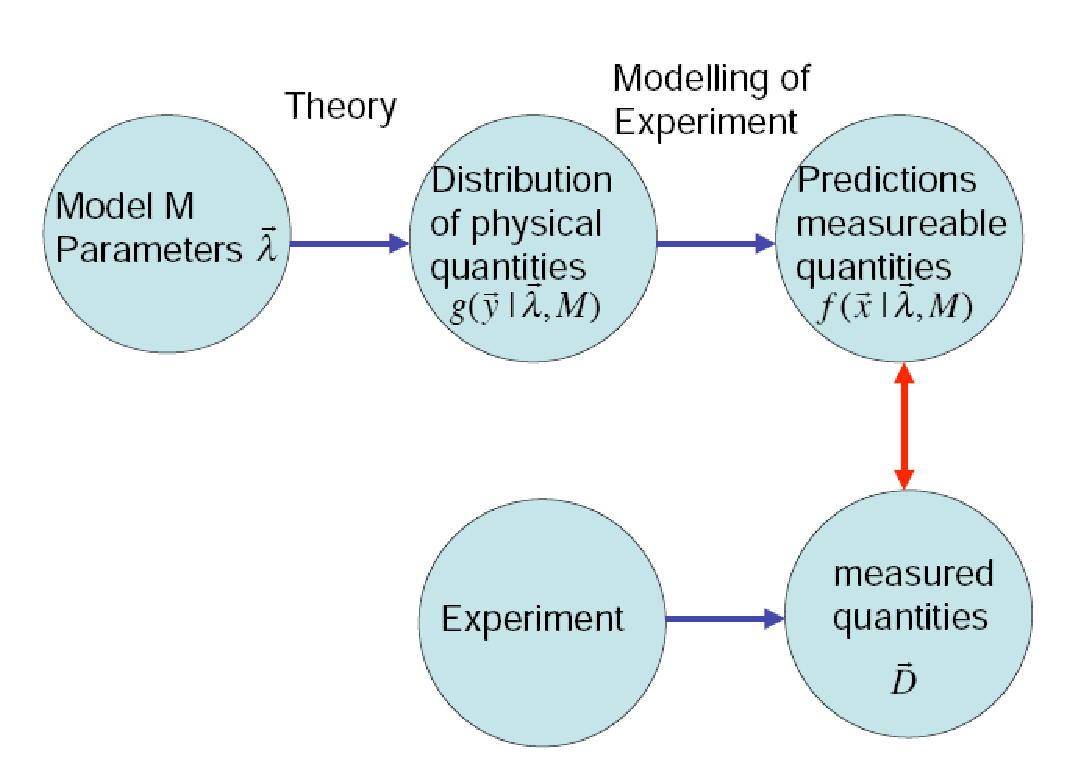
\includegraphics[width=0.75\textwidth]{scheme.eps} 
\caption{Paradigm for data analysis.  Knowledge is gained from a
comparison of model predictio ns with data.  Intermediate steps may be
necessary, e.g., to model experimental conditions.}
\label{fig:scheme}
\end{figure}

Note that the model provides `Direct Probabilities'; i.e., frequency
distributions of possible outcomes of the results were one to
reproduce the experiment many times under identical conditions.  The
function
%
\begin{equation}
f(\vec{x}|\vec{\lambda},M)
\end{equation}
%
gives the probability (density) of getting result $\vec{x}$ assuming
the model $M$ and parameters $\vec{\lambda}$\footnote{The modelling of
the experiment will usually add extra parameters and assumptions,
which then also appear as arguments}.

The probability of a model, $M$, will be quantified as $P(M)$, with:
%
\begin{equation}
\label{eq:norm}
0 \leq P(M) \leq 1
\end{equation}
%
while the probability (density) of the parameters are typically
continuous functions.  The probability (densities) satisfy
%
\begin{eqnarray*}
P(\vec{\lambda}) & \ge & 0 \\
\int P(\vec{\lambda}) d\vec{\lambda} &=&1 \;\; .\\
\end{eqnarray*}

In the Bayesian approach, the quantities $P(M), P(\vec{\lambda})$ are
treated on the same footing as the direct probabilities, although they
are not in any sense frequency distributions and must be determined
via inductive reasoning.  The procedure for learning from experiment
is:
%
\begin{equation}
P_{i+1}(\vec{\lambda},M) \propto f(\vec{x}=\vec{D}|\vec{\lambda},M) P_{i}(\vec{\lambda},M) 
\end{equation}
%
where the index represents a `state-of-knowledge'.  

In order to satisfy Eq.~\ref{eq:norm}, we set
%
\begin{equation}
P_{i+1}(\vec{\lambda},M) =\frac{f(\vec{x}=\vec{D}|\vec{\lambda},M) P_{i}(\vec{\lambda},M)}
{\sum_M \int f(\vec{x}=\vec{D}|\vec{\lambda},M) P_{i}(\vec{\lambda},M) d{\lambda}}
\end{equation}
%
We usually just write $P_i=P_0$, and this quantity is called the
`prior'.  The function $f$ does not need to be normalized, since the
overall normalization is taken care of automatically.  When $f$ is
viewed as a function of $\vec{\lambda}$ for fixed $\vec{x}=\vec{D}$,
it is known as the likelihood.

\subsection{Validity of Model}

The following quantity is proposed to evaluate the validity of a
model,$M$, (including any modelling of the experimental conditions):
%
\begin{equation}
p=\int_{f(\vec{x}|\vec{\lambda^*},M)<f(\vec{x}=\vec{D}|\vec{\lambda^*},M)} f(\vec{x}|\vec{\lambda^*},M) d\vec{\lambda}
\end{equation}
%
where $\vec{\lambda^*}$ are the optimal values of $\lambda$ (e.g.,
best-fit values). The quantity $p$ is just the `tail-area' probability
to have found any result with smaller $f$ than that given by the
measured data, given $M,\vec{\lambda^*}$.  This quantity is analogous
to the usual $\chi^2$ probability, but is more general since it can be
used for any function $f$.

\subsection{Parameter estimation}
%
Parameter estimation is performed while keeping the model fixed.  In
this case, we write
%
\begin{equation}
P_{1}(\vec{\lambda}|M) =\frac{f(\vec{x}=\vec{D}|\vec{\lambda},M) P_{0}(\vec{\lambda}|M)}
{\int f(\vec{x}=\vec{D}|\vec{\lambda},M) P_{0}(\vec{\lambda}|M) d\vec{\lambda}} \;\; .
\label{eqn:BayesTheorem}
\end{equation}
%
The output of the evaluation is a (multidimensional) normalized
probability density for the parameters, including all correlations.
This output can be used to give best-fit values, probability intervals
for the parameters, etc.

The scheme for updating knowledge, as written down here, is quite
general and straightforward.  There can be difficulties in
implementation when dealing with multi-dimensional spaces, and the
toolkit presented here is designed to help the user solve these
technical issues.  As a general statement, it should be obvious that
the `garbage in, garbage out' rule applies.  It is up to the user to
carefully define the model, parameters, predictions, and priors.  The
BAT program will then be useful as a tool for model testing and
parameter estimation.

In the following, we will give several examples of parameter
estimation and model testing to make the ideas more concrete.

% --------------------------------------------------------

\subsection{Example uses of Bayesis Inference} 
\label{subsection:exampleuses} 

Describe in general terms how a problem is formulated. Some examples:

\paragraph{Structure functions} 

\paragraph{Neutrinoless double beta-decay} 

Neutrinoless double beta-decay ($0\nu\beta\beta$) is rare nuclear
process predicted to occur if the neutrino is a Majorana
particle~\cite{Yao:2006px}. It has two electrons and no neutrinos in
the final state. Experiments searching for $0\nu\beta\beta$-decay of
$^{76}$Ge measure the ionization energy deposited in Ge-semiconductor
detectors. Since the energy released in the decay, the $Q$-value, is
fully transferred to the electrons the experimental signature of such
a decay is a sharp line at that energy. In experiments like
GERDA~\cite{Schonert:2005zn} the background in the region of interest
is expected to be flat. \\ 

\noindent 
Due to the small number of signal events predicted special care has to
be taken when analyzing the measured energy spectrum. Common
approximations which are only valid for a laarge number of events
cannot hold in that case. A spectral analysis based on Bayes' Theorem
has been developed for that purpose~\cite{Caldwell:2006yj}. The
sensitivity of the GERDA experiment has been evaluated using Monte
Carlo techniques. A simplified version of the analysis is given as an
example in the code (see Section~\ref{section:example03}). 

\paragraph{Cosmological models} 

% --------------------------------------------------------

\subsection{Requirements} 

The BAT toolkit was written to assist the user solving statistical
problems in Bayesian inference. Of course the user has to be able to
formulate the problem encountered. This means that the user has to
provide a valid model together with all parameters and limits of the
parameters. It is obvious that BAT can only help solve the
mathematical part of the statistical analysis, in particular the
numerical integration and optimization.  \\

\noindent 
During the run-time of the program the user can adjust several
parameters for numerical integration and optimization. These
parameters influence the performance of calculation and are not
connected to the mathematical formulation of the problem
encountered. In Section~\ref{section:analysis}, the steps of the
analysis chain are discussed and the adjustable parameters
introduced. It should be noted that these parameters are model
dependent and need to be adjusted to each problem separately. 

% --------------------------------------------------------
% installation 
% --------------------------------------------------------

\section{Installation} 

The BAT software package provides a library with C++ classes which can
be implemented in any other program ...

How to install BAT on your computer. Requirements, e.g. ROOT.

% --------------------------------------------------------
% analysis chain
% --------------------------------------------------------

\section{Analysis chain}
\label{section:analysis}

The following section describes the basic features and the technical
implementation of the \BAT\ toolkit. The general flow of work is the
following: one or several models are defined together with their
parameters and corresponding ranges. Data is read in from a file and
interfaced with each model. The models are then compared by
calculating the probability for each model given the data
set. Parameters are estimated either for the total probability density
or for the marginalized probability densities. Given these best-fit
parameters a ``goodness-of-fit'' can be estimated by evaluating the
posterior probability for an ensemble of possible data sets. 

% --------------------------------------------------------

\subsection{Getting started} 

The \BAT\ toolkit is meant to be used as library in any existing C++
code. In order to start a new project several files need to be
provided by the user:
% 
\begin{itemize}
\item A makefile in which the \BAT\ library is set. 
\item The include and source files of the model classes. 
\item A main file in which the actual analysis is performed. 
\end{itemize} 

% --------------------------------------------------------

\subsection{Creating a model} 

The mathematical models used in Bayesian inference are implemented in
terms of C++ classes. The basic element in this implementation is the
abstract class \verb|BCIntegrate| which contains mathematical tools
and methods. Its (only) daughter class \verb|BCModel| provides
containers for further information on the model. All model classes
inherit from the \verb|BCModel| class. It has several public methods
which need to be overloaded by the user in order to specify the
mathematical expressions for each for the three terms. Apart from the
constructor and destructor, these methods are
% 
\begin{itemize}
\item \verb|BCModel::DefineParameters()| \\
 This method has to be called at construction and contains the
 definition of parameters. 
% 
\item \verb|BCModel::LogLikelihood(std::vector <double> parameters)| \\ 
 This method contains a mathematical expression for the conditional
 probability of the data given a set of parameter values. For reasons
 of numerical stability it return the logarithm of the conditional
 probability.
%
\item \verb|BCModel::LogAPrioriProbability(std::vector <double> parameters)| \\
 This method contains a mathematical expression for the {\it a priori}
 probability for a set of parameter values. For reasons
 of numerical stability it return the logarithm of the conditional
 probability.
\end{itemize} 

\noindent 
The parameters of a model are implemented as a C++ class named
\verb|BCModelParameter|. They can be interfaced to a model in two
ways: either they are explicitly defined and then added to a model via 
%
\begin{verbatim}
BCModel::AddParameter(BCParameter * parameter) 
\end{verbatim}

\noindent 
or they are implicitly defined via 
%
\begin{verbatim}
BCModel::AddParameter(const char* name, double lowerlimit, double upperlimit) . 
\end{verbatim}

\noindent 
Every parameter has to have a unique name and valid limits. Once added
to a model the parameters can be referenced by an index or by
name. The index is given while added to the model. 
%
\begin{verbatim} 
BCModel::GetParameter(int index) 
BCModel::GetParameter(char* name) 
\end{verbatim}  

% --------------------------------------------------------

\subsection{Data format and handling} 
\label{subsection:data} 

Data is managed in the form of data points which are combined to data
sets. Data points and sets are implemented as classes
\verb|BCDataPoint| and \verb|BCDataSet|, respectively. \\ 

\noindent 
The class \verb|BCDataPoint| contains a set of double precision
values. Data points can be generated explicitly by the user with or
without intial value 
%
\begin{verbatim} 
BCDataPoint::BCDataPoint(int nvariables)
BCDataPoint::BCDataPoint(vector<double> x) 
\end{verbatim} 

\noindent 
Values of a data point can either be set value-by-value or for all
values at once
%
\begin{verbatim} 
BCDataPoint::SetValue(int index, double value)  
BCDataPoint::SetValues(std::vector <double> values) 
\end{verbatim} 

\noindent 
The value of the $i$th entry can be obtained by 
%
\begin{verbatim}
BCDataPoint::GetValue(int index); 
\end{verbatim} 

\noindent 
Data points can be added to data sets by the user via 

\begin{verbatim} 
BCDataSet::AddDataPoint(BCDataPoint* datapoint)
\end{verbatim} 

\noindent 
Alternatively, data can be read in from a file
%
\begin{small}
\begin{verbatim}
BCDataSet::ReadDataFromFileTree(char* filename, char* treename, const char* branchnames)
BCDataSet::ReadDataFromFileTxt(char* filename, int nvariables)
BCDataSet::ReadDataFromFileUser(char* filename, std::vector<int> options_int,
                                std::vector<double> options_double, const char* options_char)
\end{verbatim} 
\end{small} 

\noindent 
The format in \verb|.txt| files is chosen such that each data point
corresponds to one line each containing several values. Note, that the
number of values per data point has to be provided by the user. While
the first two methods are interfaces to pre-defined formats the third
methods allows the user to define his/her own interface. \\

\noindent 
Once a data set is defined it is assigned to a model via 
%
\begin{verbatim}
BCModel::SetDataSet(BCDataSet* dataset)
\end{verbatim} 

% --------------------------------------------------------

\subsection{Managing more than one model: the model manager} 

In case more than one model is defined and all models use the same
data set a model manager can be defined. It is implemented as a class
\verb|BCModelManager|. Models and their {\it a priori} probability are
added to the manager via
% 
\begin{verbatim}
BCModelManager::AddModel(BCModel * model, double probability)
BCModelManager::AddModel(BCModel * model)
\end{verbatim} 

\noindent 
A common data set can be defined and will be patched through to all
models added to the manager class. This can either be done explicitly
via
%
\begin{verbatim}
BCModelManager::SetDataSet(BCDataSet * dataset) 
\end{verbatim} 

\noindent 
or by reading data from a file via 
%
\begin{small}
\begin{verbatim}
BCModelManager::ReadDataFromFileTree(char* filename, char* treename, const char* branchnames)
BCModelManager::ReadDataFromFileTxt(char* filename, int nvariables)
BCModelManager::ReadDataFromFileUser(char* filename, std::vector<int> options_int,
                                std::vector<double> options_double, const char* options_char)
\end{verbatim} 
\end{small} 

% --------------------------------------------------------

\subsection{Normalization and numerical integration} 
\label{section:normalization} 

The {\it a posteriori} probability density function is normalized to
unity. To ensure this normalization the denominator on the right hand
side of Eqn.~\ref{eqn:BayesTheorem} has be to evaluated. It is an
integral of the conditional probability times the {\it a priori}
probability over the whole parameter space. Since the analytical form
of the integral is not known in general this integral is solved
numerically. Several methods for numerical integration are implemented
in the package. The different methods are described in
Section~\ref{subsection:integration}. \\

\noindent 
The integration method can be chosen for each model by 
%
\begin{verbatim}
BCIntegrate::SetIntegrationMethod(BCIntegrate::BCIntegrationType method), 
\end{verbatim} 

\noindent
where \verb|BCIntegrationType| can be one of the following 
% 
\begin{itemize}
\item \verb|BCIntegrate::kIMonteCarlo|. A sampled mean integration.
\item \verb|BCIntegrate::kIImportance|. A sampled mean integration
 with importance sampling.  
\item \verb|BCIntegrate::kIMetropolis|. A sampled mean integration
 with importance sampling using Markov chains. 
\item \verb|BCIntegrate::kICuba|. An interface to the cuba
 library~\cite{Hahn:2004fe}.
\end{itemize}

\noindent 
The time needed for the numerical integration depends on the number of
iterations. For the samples mean integration it can be constrained by
the maximum number of iterations and the relative precision aimed
at. These parameters can be set via
%
\begin{verbatim}
BCIntegrate::SetNIterationsMax(int niterations)
BCIntegrate::SetRelativePrecision(double relprecision) 
\end{verbatim} 

\noindent 
For all other methods the number of iterations is explicitly set via 
%
\begin{verbatim}
BCIntegrate::SetNiterationsPerDimension(int niterations) 
\end{verbatim} 

\noindent 
The integration can be performed for each model separately or for all models which belong to a model manager 
%
\begin{verbatim}
BCModel::Normalize() 
BCModelManager::Initialize()
\end{verbatim} 

\noindent 
The private variable \verb|fNormalization| is set for each model. Once
the integral is calculated the {\it a posteriori} probability for a
set of parameter values can be evaluated

\begin{verbatim} 
BCModel::Probability(std::vector <double> parameter) .  
\end{verbatim} 

% --------------------------------------------------------

\subsection{Hypothesis testing and model comparison} 

Several models or hypotheses can be compared. These models are added
to a model manager and given an {\it a priori} probability. The {\it a
posteriori} probability for each model with respect to the whole set
of models is calculated. The posterior probability for the $i$th
model, $H_{i}$, given the data, is simply
%
\begin{equation}
p(\mathrm{H_{1}}|\mathrm{data}) = \frac{N_{1} \cdot p_{0}(H_{1})}{\sum_{i = 1}^{N} N_{i} \cdot p_{0}(H_{i})} \, , 
\end{equation}
%
where $N_{i}$ is the normalization of the $i$th model posterior
probability (i.e. the denominator of the right hand side of
Eqn.~\ref{eqn:BayesTheorem}) and $p_{0}(H_{i})$ is the prior
probability for the $i$th model. \\ 

\noindent 
The model {\it a posteriori} probability can be evaluated once the
model manager is initialized and all numerical integrations are
performed
%
\begin{verbatim}
BCModel::GetModelAPosterioriProbability()
\end{verbatim}

% --------------------------------------------------------

\subsection{Parameter estimate and marginalization} 

The {\it a posteriori} probability can be used to estimate the set of
parameter values most suited to describe the data. This is done by
searching for the most probable value, or mode of the
distribution. Two approaches are followed: either the mode in the
whole parameter space is searched for, or the probability density is
marginalized with respect to the parameter under study. The former
case can be realized by 
%
\begin{verbatim} 
BCModel::FindMode()
\end{verbatim} 

\noindent 
which returns a vector of parameter values which maximize the {\it a
posteriori} probability density. The algorithm used is described in
Section~\ref{section:tools}. \\ 

\noindent 
The single parameter estimate is done by marginalization. If more than
one parameter is studied it is most efficient to marginalize with
respect to all parameters simultaneously. This can be done by
%
\begin{verbatim}
BCModel::MarginalizeAll() 
\end{verbatim} 

\noindent 
A vector of one- and two-dimensional histograms is filled during the
marginalization and can be accessed by
%
\begin{verbatim}
BCModel::GetMarginalized(BCParameter * parameter) 
BCModel::GetMarginalized(char * name) 
BCModel::GetMarginalized(BCParameter * parameter1, BCParameter * parameter2) 
BCModel::GetMarginalized(char * name1, char * name2) 
\end{verbatim}

\noindent 
Alternatively, the marginalization can be done for one or two
parameters separately
%
\begin{verbatim}
BCModel::MarginalizeProbability(BCParameter* parameter)
BCModel::MarginalizeProbability(char* name) 
BCModel::MarginalizeProbability(BCParameter * parameter1, BCParameter * parameter2);
BCModel::MarginalizeProbability(char * name1, char * name2)
\end{verbatim} 

\noindent 
Different methods of marginalization are implemented and be chosen via
%
\begin{verbatim}
BCIntegrate::SetMarginalizationMethod(BCIntegrate::BCMarginalizationType method)
\end{verbatim} 

\noindent
where \verb|BCMarginalizationType| can be one of the following 
% 
\begin{itemize}
\item \verb|BCIntegrate::kMMonteCarlo|. Uncorrelated sampling of the
 probability density.  
\item \verb|BCIntegrate::kMMetropolis|. Correlated sampling using
 Markov chains.
\end{itemize} 

\noindent 
The different methods are described in
Section~\ref{subsection:optimization}. Note, that if the
marginalization is done for all parameters simultaneously only Markov
chains can be used. \\

% --------------------------------------------------------

\subsection{One- and two-dimensional histograms} 

The classes \verb|BCH1D| and \verb|BCH2D| are one- and two-dimensional
histgram classes which inherit from the ROOT-classes \verb|TH1D| and
\verb|TH2D|. The mean and mode of a distribution can be obtained by 
%
\begin{verbatim}
BCH1D::GetMean()
BCH1D::GetMode()
BCH2D::GetMean()
BCH2D::GetMode()
\end{verbatim} 

\noindent 
The one-dimensional histogram can also return the uncertainty on the
parameter defined as the region from 16\% to 84\% probability seen
from the mean or mode
%
\begin{verbatim}
GetUncertaintyPlusFromMean()
GetUncertaintyMinusFromMean()
GetUncertaintyPlusFromMode()
GetUncertaintyMinusFromMode()
\end{verbatim} 

\noindent 
Also, the one-dimensional histograms have methods to return the
quantiles and the 90\%, 95\% and 99\% exclusision limits
%
\begin{verbatim} 
BCH1D::GetQuantile (double probabilitysum)
BCH1D::GetLimit90()
BCH1D::GetLimit95()
BCH1D::GetLimit99()
\end{verbatim} 

\noindent 
In addition, the smallest interval containing a certain probability
can be obtained for a one-dimensional histogram 
%
\begin{verbatim}
BCH1D::GetSmallestInterval(double & min, double & max, double content=.68) . 
\end{verbatim}

\noindent 
Both type of histograms can be printed to an \verb|.eps| or \verb|.ps|
file via

\begin{verbatim}
BCH1D::Print(char * filename, int options=0, double ovalue=0.)
BCH2D::Print (char *filename, int options)
\end{verbatim}  

The printing options are summarized in Table~\ref{table:printingoptions}. 

\begin{table}[ht!]
\begin{tabular}{ll}
\hline
Option & Style \\ 
\hline
BCH1D & \\ 
\hline 
0 (default) & \begin{minipage}[l]{12 cm}Draws a colored band at the central 68\% probability region. If the mode is not inside this band, the 95\% probabilty limit is drawn. \end{minipage}\\ 
1           & Draws a line at the value passed. \\ 
2           & Draws a colored band at the smallest interval containing \verb|ovalue|\% probability. \\
\hline 
BCH2D & \\ 
\hline 
0 (default) & Draw with the ROOT option \verb|CONT0|. \\ 
1           & Draw the 68\%, 95\% and 99\% probability contours. \\ 
2           & Draw the 68\% probability contour. \\ 
3           & Draw the 90\% probability contour. \\ 
4           & Draw the 95\% probability contour. \\ 
\hline
\end{tabular}
\caption{Printing options for one- and two-dimensional histograms. 
\label{table:printingoptions}} 
\end{table}

\pagebreak 

% --------------------------------------------------------

\subsection{Posterior probability check: a goodness-of-fit test} 

Once the most suited parameter set, $\lambda^{*}$, for a given model
and data set, $D$, is estimated the quality of the model with this
parameter set can be tested. This ``goodness--of-fit'' test is based
on a set of fake data sets, $\{ \tilde{D} \}$, generated under the
assumption of the parameters obtained, $\lambda^{*}$. A frequency
distribution $f$ of the obtained conditional probability
$k=p(\tilde{D}|\lambda^{*})$ is calculated and interpreted as
probability density. The $p$-value is defined as the probability to
find a conditional probability $p(\tilde{D}|\lambda^{*})$ equal or
larger than for the original data set, $k_{0}=p(D|\lambda^{*})$, i.e.
%
\begin{equation}
p = \frac{1}{n} \int_{k_{0}=p(D|\lambda^{*})}^{1} f(k) \, \mathrm{d}k 
\end{equation} 

\noindent 
The user has to provide data sets the generated with the parameter set
$\lambda^{*}$. Each data set has to be written to a separate text file
with the format described in Section~\ref{subsection:data}. A file
containing a list of data set files has to be provided. The
goodness-of-fit test is done by calling
%
\begin{verbatim}
BCModel::GoodnessOfFitTest(const char * filenname, std::vector <double> parameters) 
\end{verbatim} 

\noindent 
The method returns a pointer to a \verb|BCH1D|. The frequency
distribution can be printed as for the case of parameter
estimates. The $p$-value is then calculated from this distribution and
can be obtained by 
%
\begin{verbatim}
BCModel::GetPValue() . 
\end{verbatim} 

% --------------------------------------------------------

\subsection{Summary} 

During any time of the analysis the model manager can print a summary
of models, their parameters and results obtained so far for
optimization. 
%
\begin{verbatim}
BCModel::PrintSummary(char * filename=0)
\end{verbatim} 

\noindent 
The summary is written to a file. In case no filename is specified the
summary is printed onto the screen. 

% --------------------------------------------------------
% technical tools 
% --------------------------------------------------------

\section{Technical tools} 
\label{section:tools} 

% --------------------------------------------------------

\subsection{The log book} 

The class \verb|BCLog| is used to write out information during the
runtime of program. The output is written to screen and to a log
file. The minimum level of detail can be set by the user via
%
\begin{verbatim} 
SetMinimumLogLevelFile(BCLog::LogLevel loglevel)
SetMinimumLogLevelScreen(BCLog::LogLevel loglevel)
\end{verbatim} 

\noindent 
where the level is one of the following 
%
\begin{itemize} 
\item \verb|debug|: Lowest level of information. 
\item \verb|detail|: Details of functions, etc. 
\item \verb|summary|: Results such as best-fit values, etc. 
\item \verb|warning|: Warning messages 
\item \verb|nothing|: Nothing is written out. 
\end{itemize} 

The user has to open a log file in the beginning using 
%
\begin{verbatim} 
BCLog::OpenLog() . 
\end{verbatim} 

% --------------------------------------------------------

\subsection{Optimization} 
\label{section:optimization} 

Describe how optimization is done, etc. It should be clear what
parameters can be controlled by the user and what they mean.

% --------------------------------------------------------

\subsection{Numerical integration} 
\label{section:integration} 

The different methods of numerical integration are shortly discussed
in the following. The basic idea of Monte Carlo integration is that an
integral can be approximated with a finte sum. For a function $f$
defined between~0 and~1 this yields 
% 
\begin{equation}
\int_{0}^{1} f(x) \, \mathrm{d}x \approx \frac{1}{N} \sum_{i=1}^{N} f(x_{i}) \, , 
\label{eqn:integration}
\end{equation} 

\noindent 
where $N$ is the number of samples. The values $x_{i}$ are randomly
sampled from a uniform distribution. The statistical uncertainty the
expression goes as $1/\sqrt{N}$ independent of the dimension. 

\paragraph{Sampled mean integration} 

The sampled mean integation is the simplest implementation of Monte
Carlo integration. It uses the approximation from
Eqn.~\ref{eqn:integration} for arbitrary limits of parameters, thus
including a Jacobian term, $J$:
%
\begin{eqnarray}
\int_{a}^{b} f(x) \, \mathrm{d}x & = & \int_{0}^{1} f(x) \cdot J(x) \, \mathrm{d}x \\ 
                                 & = & \int_{0}^{1} f(x) \cdot (b - a) \, \mathrm{d}x \\ 
				 & \approx & \frac{(b - a)}{N} \sum_{i=1}^{N} f(x_{i}) =: \mu
\end{eqnarray} 

\noindent 
The uncertainty of the integral is the standard deviation of the mean
value and thus 
%
\begin{equation}
\sigma_{\mu} = \frac{1}{\sqrt{N}} \cdot \sqrt{\overline{x^{2}} - \overline{x}^{2}} \, . 
\end{equation} 

\noindent 
The number of samples is limited to a maximum. If the relative
precision, $\sigma_{\mu}/\mu$ is less than a chosen value, the
sampling stops (see Section~\ref{section:normalization}). 

\paragraph{Sampled mean integration with importance sampling} 

Instead of sampling from a uniform distribution a well known function
can be used as underlying distribution for the $x_{i}$. The integral
from Eqn.~\ref{eqn:integration} is then computes as 
%
\begin{eqnarray}
\int_{a}^{b} f(x) \, \mathrm{d}x & = & \int_{a}^{b} \frac{f(x)}{g(x)} \cdot g(x) \cdot J(x) \, \mathrm{d}x \\ 
 & \approx & \frac{(b - a)}{N} \sum_{i=1}^{N} \frac{f(x_{i})}{g(x_{i})} \, , 
\end{eqnarray} 

\noindent 
where the $x_{i}$ are sampled according to $g$. Note, that $g$ has to
be normalized to unity. \\ 

\noindent 
The number of iterations has to be set directly (see Section~\ref{section:normalization}). 

\paragraph{Sampled mean integration with importance sampling using Markov chains} 

Instead of using uncorrelated numbers of $x$ values in the importance
sampling, Markov chain can be used. Regions of higher probability are
found faster and the statistical fluctuation descreases. For more
details on Markov chains, see Section~\ref{section:optimization}.

% --------------------------------------------------------
% examples
% --------------------------------------------------------

\section{Examples}

Several examples are provided together with the \BAT\ libraries. These
are discussed in the following. 

% --------------------------------------------------------

\subsection{Example 01: Straight line fit} 

In the first example the basic problem of fitting a straight line to a
set of measured points is addressed. The data set consists of data
points of a measured quantity $y$ at fixed $x$ values with some
uncertainty $\sigma_{y}$. The model assumes a linear correlation
between $x$ and $y$ where the uncertainty on the measured $y$ is
assumed to be Gaussian with the given uncertainty~$\sigma_{y}$. The
two parameters of the model are the slope and offset describing the
linear curve. \\

\noindent 
First, the main program file, \verb|runBAT.c| is discussed. Then, the
two files describing the underlying model are shown. \\ 

\pagebreak 

\paragraph{The main program file} 
% 
\begin{small} 
\begin{verbatim}
#include <BCModelPol1.h>
#include <BCLog.h> 

int main()
{
  // open a new log book 

  BCLog::OpenLog(); 

  // create an instance of the model defined in BCModelPol1.h 
  // which describes a linear correlation between a set of 
  // data points. 

  BCModelPol1* fModelPol1 = new BCModelPol1("ModelPol1"); 

  // create a new data set 

  BCDataSet* fDataSet = new BCDataSet(); 

  // read the data from a .txt file. The three components of each 
  // data point are values for x, y and the uncertainty on y. 

  if (fDataSet -> ReadDataFromFileTxt("./data/data.txt", 3) != 0)
    return -1; 

  // assign the data set to the model 

  fModelPol1 -> SetDataSet(fDataSet); 

  // perform the mode finding using a simulated annealing. 

  fModelPol1 -> FindMode(); 

  // set number of bins in the marginalized histogram 

  fModelPol1 -> SetNbins(50);

  // perform the marginalization with respect to all parameters 
  // simultaneously. The resulting histograms are saved in a 
  // private vector of histograms. 

  fModelPol1 -> MarginalizeAll();

  // return the one-dimensional histograms of the marginalized 
  // probability density and print them to a .ps file. The 
  // default option (shaded band of the central 68\% probability) 
  // is used. 

  fModelPol1 -> GetMarginalized("constant") -> Print("modelpol1_constant.ps");
  fModelPol1 -> GetMarginalized("slope") -> Print("modelpol1_slope.ps");

  // return the two-dimensional histogram of the marginalized 
  // probability density and print it to a .ps file. The 
  // option 2 (contour containing 68\% probability) is used. 

  fModelPol1 -> GetMarginalized("constant", "slope") 
	     -> Print("modelpol1_constant_slope.ps", 2);

  // print a summary of the model and its parameters together 
  // with the best fit values to screen. 

  fModelPol1 -> PrintSummary(); 
} 
\end{verbatim} 
\end{small} 

\pagebreak 

\paragraph{The include file} 
% 
\begin{small} 
\begin{verbatim}
#include "BCModel.h" 

// create a new class which inherits from BCModel. 

class BCModelPol1 : public BCModel 
{
 public: 

  // constructors 

  BCModelPol1(); 

  BCModelPol1(const char* name); 

  // destructor 

  ~BCModelPol1()
    { ;};  

  // a method which defines the parameters and adds them to 
  // the model. 

  void DefineParameters(); 

  // the overloaded method which returns the logarithm of the 
  // conditional probability for a certain set of parameter 
  // values. 

  double LogLikelihood(std::vector <double> parameters); 

  // the overloaded method which returns the logarithm of the 
  // a priori probability for a certain set of parameter 
  // values. 

  double LogAPrioriProbability(std::vector <double> parameters); 
}; 
\end{verbatim} 
\end{small} 

\pagebreak 

\paragraph{The model file} 
% 
\begin{small} 
\begin{verbatim}
#include "BCModelPol1.h" 

#include <TMath.h> 

BCModelPol1::BCModelPol1() : BCModel()
{
  // define the parameters at the construction of the instance 

  this -> DefineParameters();
}

BCModelPol1::BCModelPol1(const char* name) : BCModel(name)
{
  // define the parameters at the construction of the instance 

  this -> DefineParameters();
}

void BCModelPol1::DefineParameters()
{
  // define two parameters which describe a straight line: 
  // 0: a constant with values in the interval [1.0, 3.0] 
  // 1: a slope with values in the interval [0.0, 0.03]
  // The parameters can be references either via their names 
  // or via their index. 

  this -> AddParameter("constant", 1.0, 3.0);  // index 0
  this -> AddParameter("slope",    0.0, 0.03); // index 1
}

double BCModelPol1::LogAPrioriProbability(std::vector <double> parameters)
{
  // the a priori probability is assumed to be flat with respect 
  // to the two parameters 

  // get the range for the parameter constant (index 0) 

  double offset_lower = this -> GetParameter(0) -> GetLowerLimit();
  double offset_upper = this -> GetParameter(0) -> GetUpperLimit();

  // get the range for the parameter slope (index 1) 

  double slope_lower = this -> GetParameter(1) -> GetLowerLimit();
  double slope_upper = this -> GetParameter(1) -> GetUpperLimit();

  // calculate the natural logarithm of the flat probability

  double logprob = 0.;
  logprob -= TMath::Log(offset_upper - offset_lower);
  logprob -= TMath::Log(slope_upper - slope_lower);

  // return the logarithm of the a priori probability 

  return logprob;
}

double BCModelPol1::LogLikelihood(std::vector <double> parameters)
{
  // the conditional probability is calculated from the product 
  // of n Gaussians, where n is the number of data points. 

  // define log of probability

  double logprob = 0.0;

  // get parameter values

  double offset = parameters.at(0);
  double slope  = parameters.at(1);

  // loop over all data points

  int npoints = this -> GetNDataPoints();

  for (int ipoint = 0; ipoint < npoints; ipoint++)
    {
      // define data values

      double x       = this -> GetDataPoint(ipoint) -> GetValue(0);
      double y       = this -> GetDataPoint(ipoint) -> GetValue(1);
      double sigma_y = this -> GetDataPoint(ipoint) -> GetValue(2);

      // calculate probability assuming a Gaussian distribution for each point
 
      logprob += BCMath::LogGaus(y, (offset + x * slope), sigma_y, true);
    }

  // return the logarithm of the conditional probability 

  return logprob; 
}
\end{verbatim} 
\end{small} 

\noindent 
Fig.~\ref{fig:example01} (left) shows the data set used in the example
and the best-fit straight line. The same figure (middle) shows the
two-dimensional contour of the parameters containing 68\% probability
and the global best-fit results. Fig.~\ref{fig:example01} (right)
shows the marginalized probability density for the parameters
\verb|constant| together with the mode and the central 68\%
probability region.

\begin{figure}[ht!]
\begin{tabular}{ccc}
\begin{minipage}[t]{0.3\textwidth}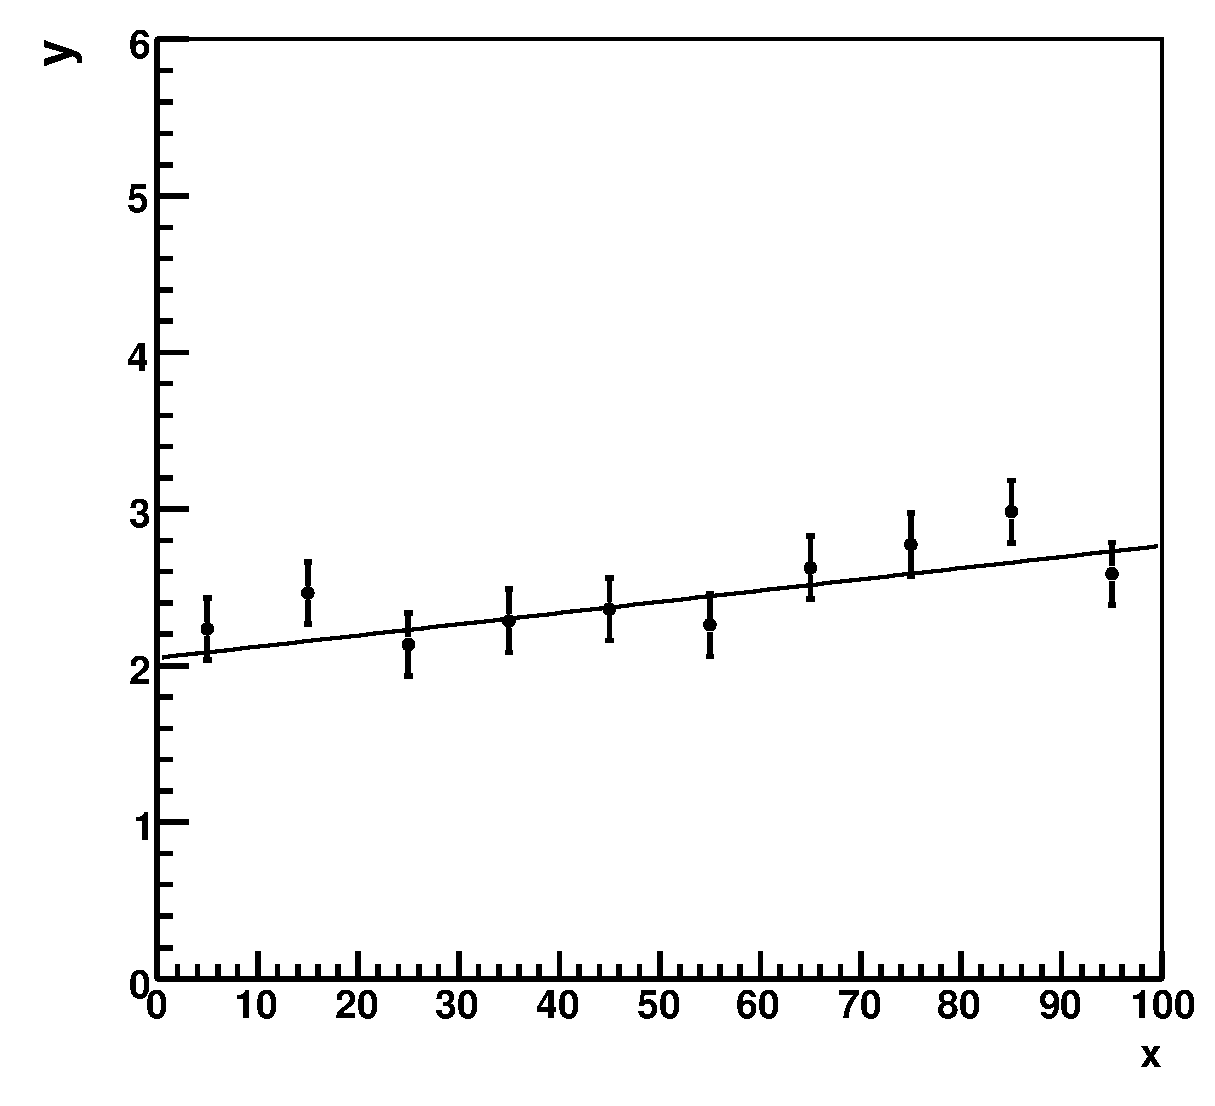
\includegraphics[height=4.0cm]{example01_data.eps}\end{minipage} & 
\begin{minipage}[t]{0.3\textwidth}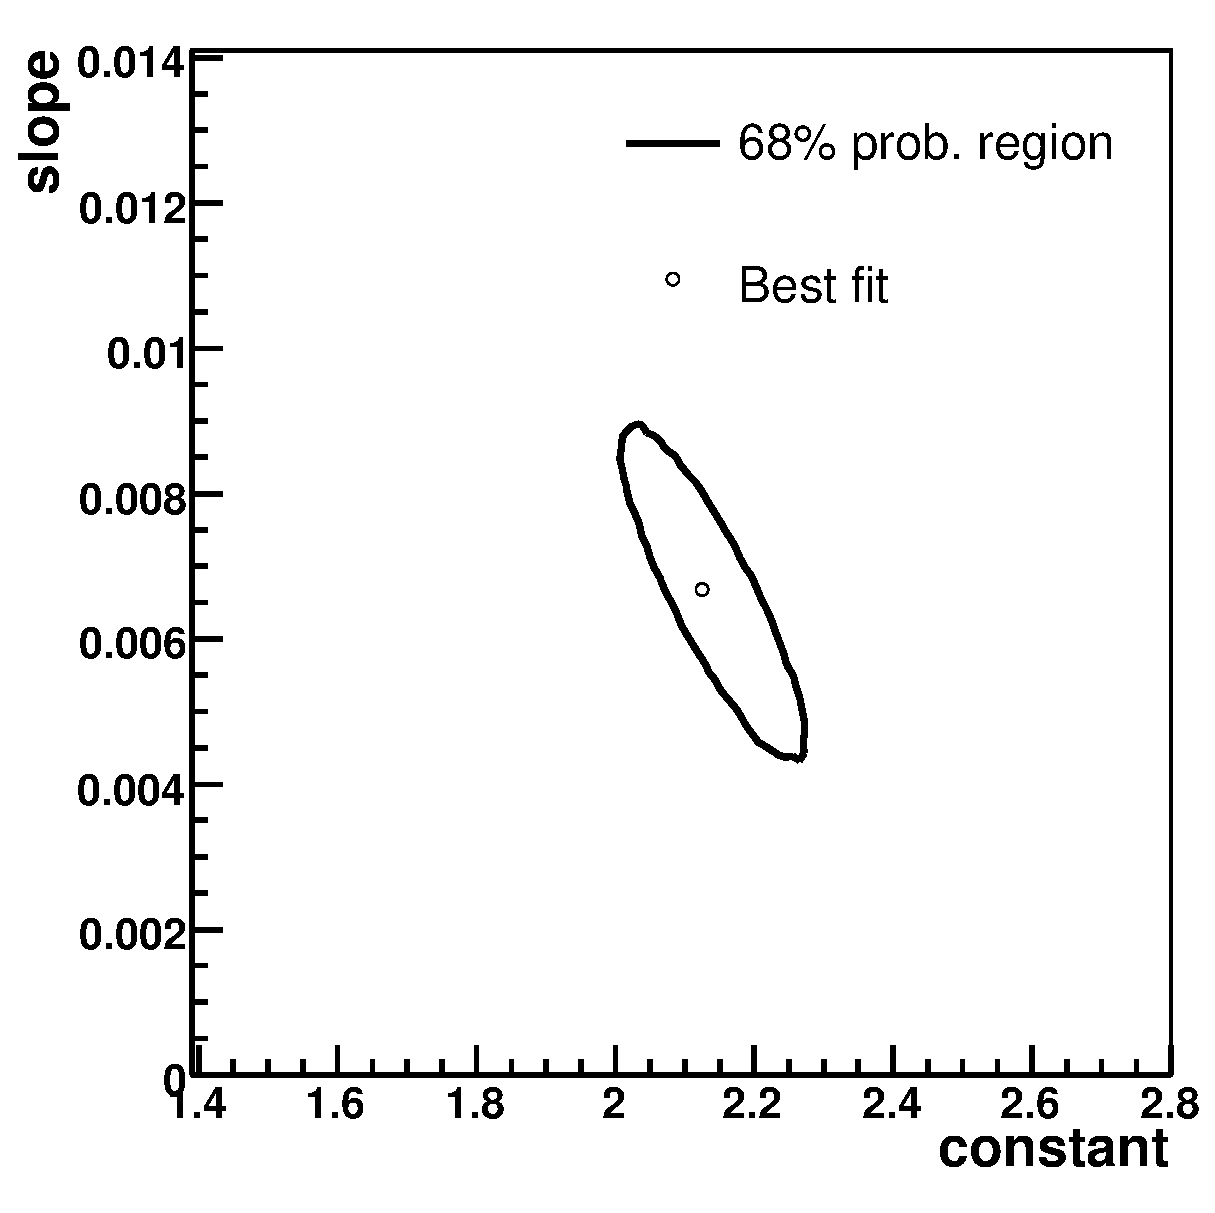
\includegraphics[height=4.0cm]{example01_correlation.eps}\end{minipage}  &
\begin{minipage}[t]{0.3\textwidth}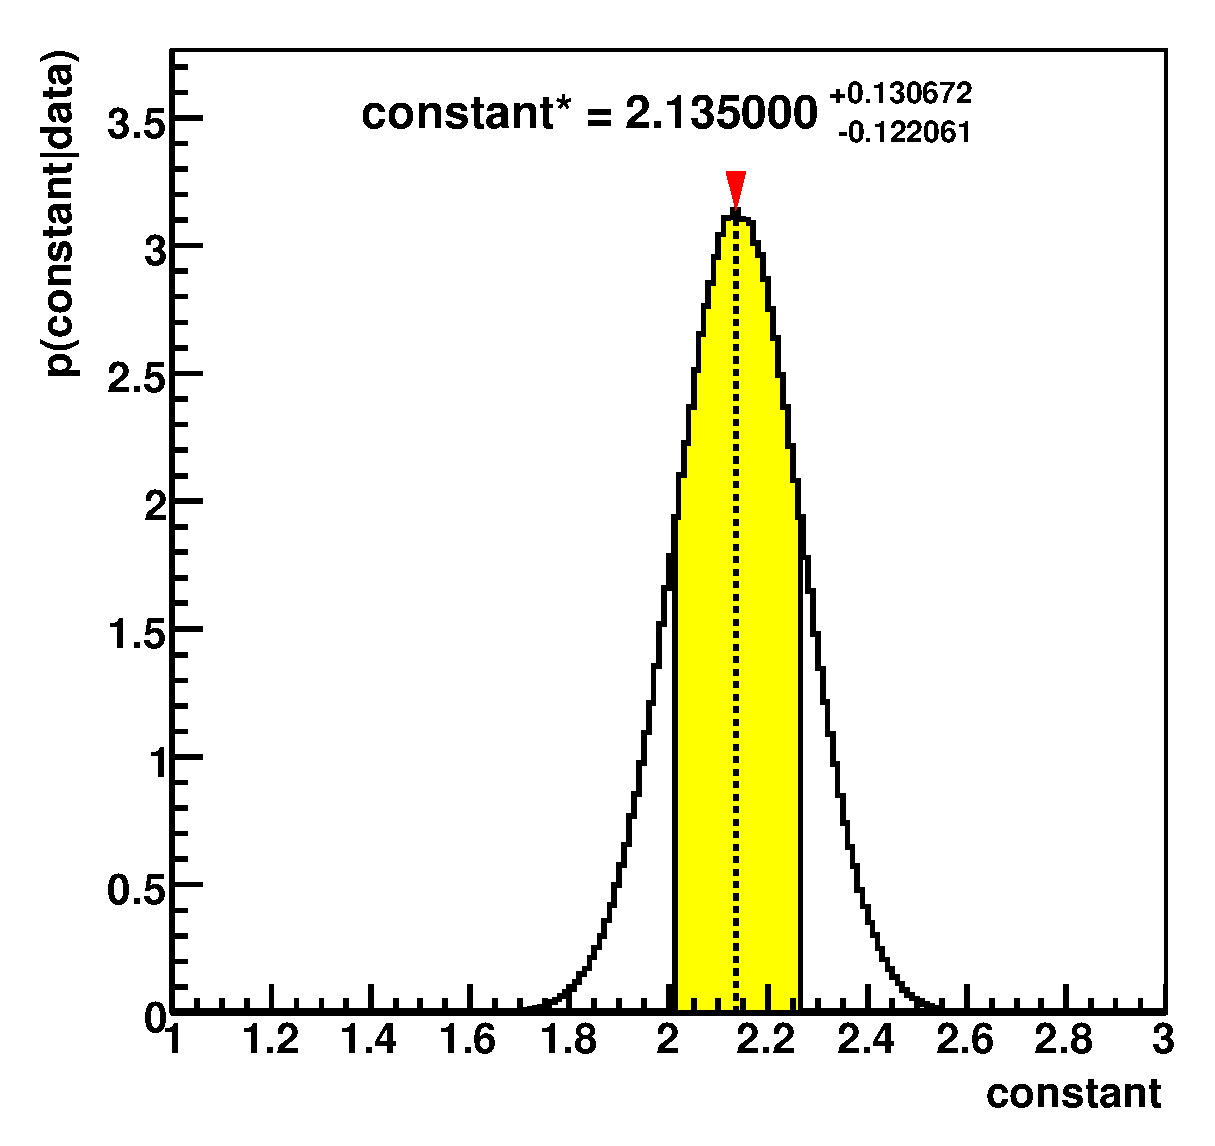
\includegraphics[height=4.0cm]{example01_constant.eps}\end{minipage} 
\end{tabular}
\caption{Left: Data set used in the example01 and best-fit straight line. Middle: Contour containing 68\% probability. Right: Marginalized probability density for the parameter constant. 
\label{fig:example01}}
\end{figure}

% --------------------------------------------------------

\subsection{Example 02: Polynomial fitting} 

As an extension of example~01 three different models are compared to
describe the data set. The difference between the model is the order
of the polynomial describing the correlation between the points:
constant, linear, quadratic. All three models are fitted to the data
and the a posteriori probability for the models is calculated. A
goodness-of-fit test is performed for the most probable model.

% --------------------------------------------------------

\subsection{Example 03: Spectral analysis} 
\label{section:example03} 

The data set is a binned spectrum with independent Poissonian
fluctuations in each bin. Two models for The underlying distribution
are compared: a background only distribution which is flat, and a
signal distribuion which has, in addition to a flat background, a
Gaussian peak at a defined position and with defined width. In the
former case, only the amount of background is a parameter while in the
latter case both, signal and background contribution, are parameters. 

% --------------------------------------------------------

\subsection{Example 04: Efficiency calculation} 

Given two numbers, $n$ and $k$, an efficiency is calculated as the
ratiom, $k/n$, of the two numbers. The one model implemented assumes
Poissonian fluctuations on $n$ and a Binomial distribution on $k$
given $n$. 

% --------------------------------------------------------
% bibliography 
% --------------------------------------------------------

\addcontentsline{toc}{section}{Bibliography}

\begin{thebibliography}{99}
%
\bibitem{Yao:2006px}
  W.~M.~Yao {\it et al.}  [Particle Data Group],
  ``Review of particle physics,''
  J.\ Phys.\ G {\bf 33} (2006) 1.
%
\bibitem{Schonert:2005zn}
  S.~Sch\"onert {\it et al.}  [GERDA Collaboration],
  ``The GERmanium Detector Array (GERDA) for the search of neutrinoless beta
  beta decays of Ge-76 at LNGS,''
  Nucl.\ Phys.\ Proc.\ Suppl.\  {\bf 145} (2005) 242.
%
\bibitem{Caldwell:2006yj}
  A.~Caldwell and K.~Kr\"oninger,
  ``Signal discovery in sparse spectra: A Bayesian analysis,''
  Phys.\ Rev.\  D {\bf 74}, 092003 (2006)
  [arXiv:physics/0608249].
%
\bibitem{Hahn:2004fe}
  T.~Hahn, ``CUBA: A library for multidimensional numerical
  integration,'' Comput.\ Phys.\ Commun.\ {\bf 168} (2005) 78
  [arXiv:hep-ph/0404043].
\end{thebibliography}


\end{document} 


